\section{分类问题}
\subsection{由回归到分类}
对于二元分类问题,一个自然的想法是当做回归问题求解,对于一类样本,令函数目标值为1,另一类目标值为-1。这在两类样本分布合理情况下是可以做到的,但是当样本分布差异很大时,从回归的角度思考就会出现问题。如图\ref{fig:ref_to_classification}所示:
\begin{figure}
	\centering
	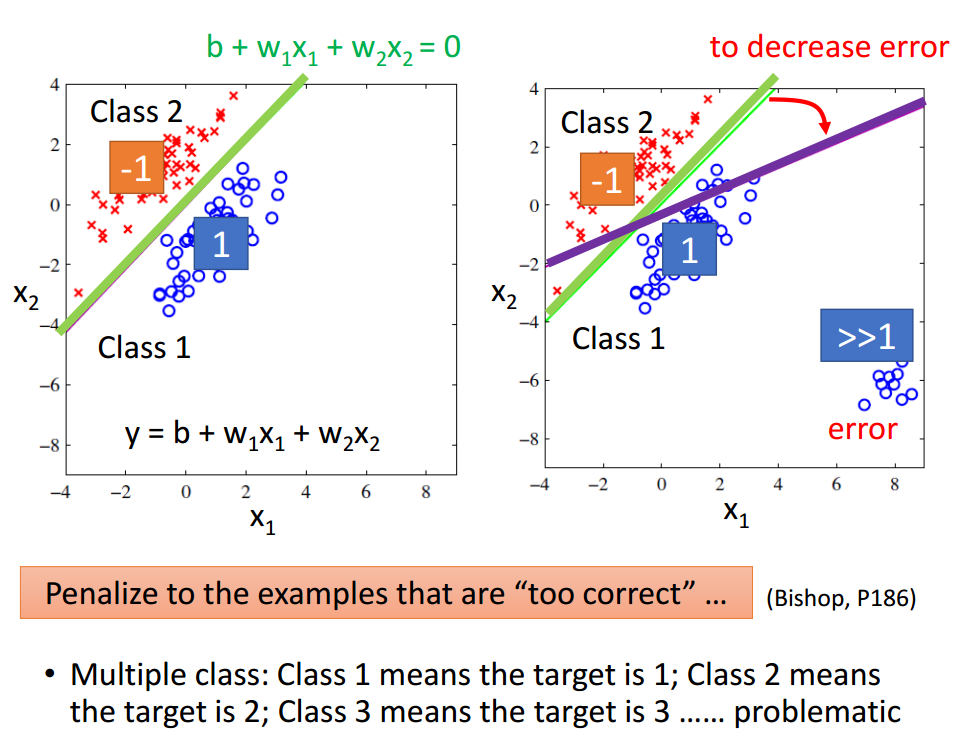
\includegraphics[scale=0.5]{pic/regression_to_classification.png}
	\caption{不合理的分布导致回归求解分类问题时出错}
	\label{fig:ref_to_classification}
\end{figure}
右下角的异常点导致回归得到边界线是紫色线,出现错误。而对于多类分类问题,依旧尝试使用回归求解,如类别1、2、3分别赋予目标值1、2、3则是不行的。